\documentclass{beamer}
\mode<presentation>
{
  \usetheme[headline]{ICL}
  % or ...

  \setbeamercovered{transparent}
  % or whatever (possibly just delete it)
}
%\setbeamertemplate{headline}[default]
%\setbeamercovered{transparent}
%\setbeamertemplate{footline}[default]
%\setbeamertemplate{headline}[split]
\usepackage[T1]{fontenc}
\usepackage[utf8]{inputenc}
\usepackage{times}
\usepackage[english]{babel}
\usepackage{color}  
\usepackage{pifont}
\usepackage{multicol}
\usepackage{multirow}
\usepackage{pgf}
\usepackage{graphicx}
\usepackage{hyperref}
%\usepackage{algorithm}
%\usepackage{algorithmic}
\usepackage{xspace}
\usepackage{transparent}

%%%%%%%%%definition des variables%%%%%%%%%%%%%%%
%\usepackage[latin1]{inputenc}
%\usepackage[T1]{fontenc}
%\usepackage{textcomp}
%\usepackage{lmodern}
%\usepackage{listings} 


%%%%%%%%%%%%%%%%%%%%%%%%%%%%%
\def\sujet{}
\def\projet{LU Decompositions over DAGuE} 
\def\etape{}
\def\gA{Omar \textsc{Zenati}, MsC Candidate}
\def\gB{Supervisors: M. Faverge, E. Agullo, G. Bosilca, P. Ramet}



%%%%%%%%%%%%%%%% Header %%%%%%%%%%%%%%%%
 \title[LU Decompositions over DAGuE]{
        {\bfseries \projet\\} 
        {\bfseries \huge \sujet}
        {\small Friday Lunch Talk}
}


\titlegraphic{
  
\includegraphics[scale=0.5]{icl.png}
  \hfill
  
\includegraphics[scale=0.3]{inria.png}
  }
\date{May 25, 2012}

\author[Zenati]{
  {\normalsize \bfseries \sffamily} {\large \gA}\\
  \vspace{1cm}
  {\normalsize \bfseries \sffamily} {\large \gB}\\
}


\AtBeginSection[]{
  \begin{frame}{Summary}
  \tableofcontents[currentsection,subsectionstyle=shaded]
  \end{frame}
}

\AtBeginSubsection[]{
  \begin{frame}{Summary}
  \tableofcontents[currentsection,currentsubsection]
  \end{frame}
}
\begin{document}

\begin{frame}
\maketitle
\end{frame}

\begin{frame}{Summary}
\tableofcontents
\end{frame}


\section[LU Algorithms]{LU Decomposition Algorithms}
\begin{frame}{Introduction}
\begin{itemize}
\item The evolution (linpack, lapack, scalapack, plasma, dplasma)
\end{itemize}
\end{frame}

\begin{frame}{Introduction}
\begin{itemize}
\item Static algorithm:
\begin{itemize}
\item Without pivoting
\item Static pivoting
\item Incremental pivoting
\end{itemize}
\item Dynamic algorithm:
\begin{itemize}
\item Partial pivoting
\item Total pivoting
\end{itemize}
\end{itemize}
\end{frame}

\section[DAGuE]{DAGuE Runtime System}
\begin{frame}{DAGuE}
\framesubtitle{Quick presentation}
\begin{center}
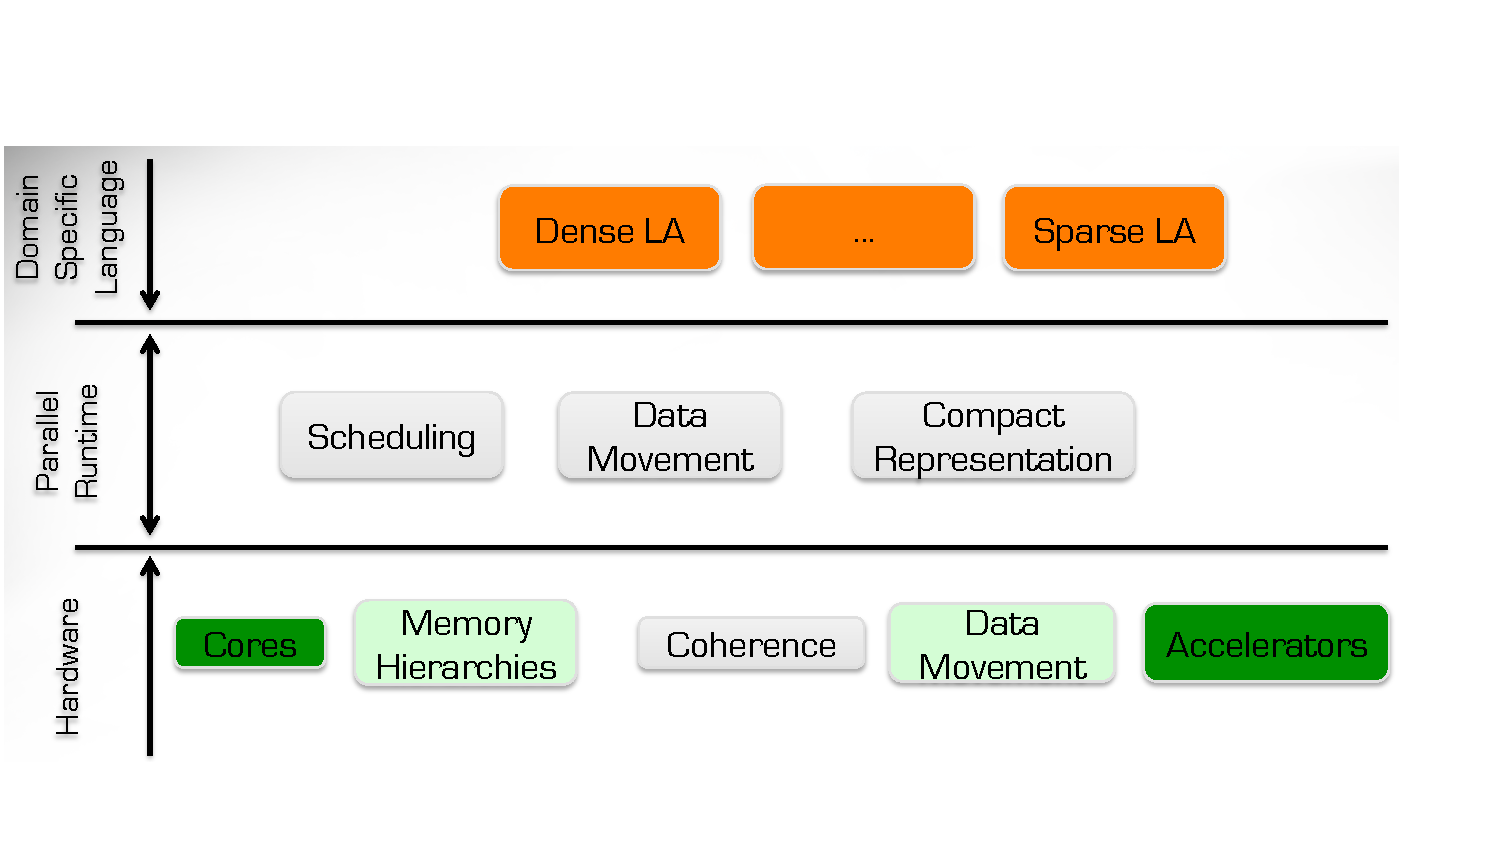
\includegraphics[scale=0.5]{3layer.pdf}
\end{center}
\end{frame}

\begin{frame}{DAGuE}
\framesubtitle{Quick presentation}
DAGuE is a Direct Acyclic Graph scheduler Engine based on task flow model where :
\begin{itemize}
\item nodes are tasks
\item edges are dependancies
\end{itemize}
\begin{center}
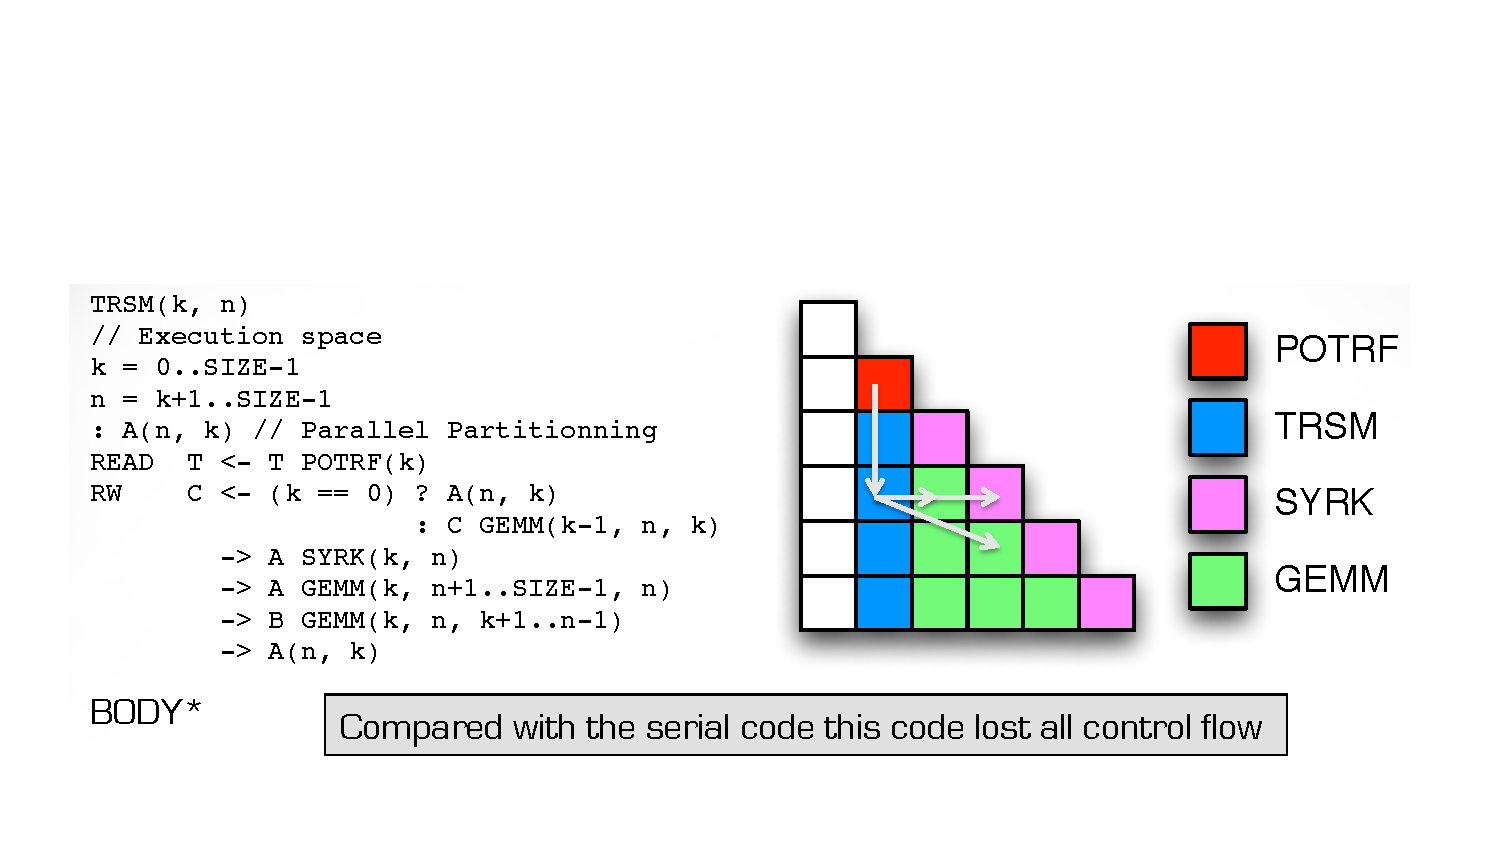
\includegraphics[scale=0.5]{trsm.pdf}
\end{center}
\end{frame}

\begin{frame}{DAGuE}
\begin{exampleblock}{Advantages :}
\begin{itemize}
\item Independence between performances and computers
\item Provide multicore parallelism
\item Good reactivity for load imbalance
\item Natural look ahead
\end{itemize}
\end{exampleblock}{}
\pause
\begin{exampleblock}{Problems :}
\begin{itemize}
\item DAG is a static representation of a task flow
\end{itemize}
\end{exampleblock}{}
\end{frame}



\section{Static Pivoting}
\begin{frame}{Static Pivoting}
\framesubtitle{Motivation}
\end{frame}

\begin{frame}{Static Pivoting}
\framesubtitle{Algebraic Representation}
\begin{center}
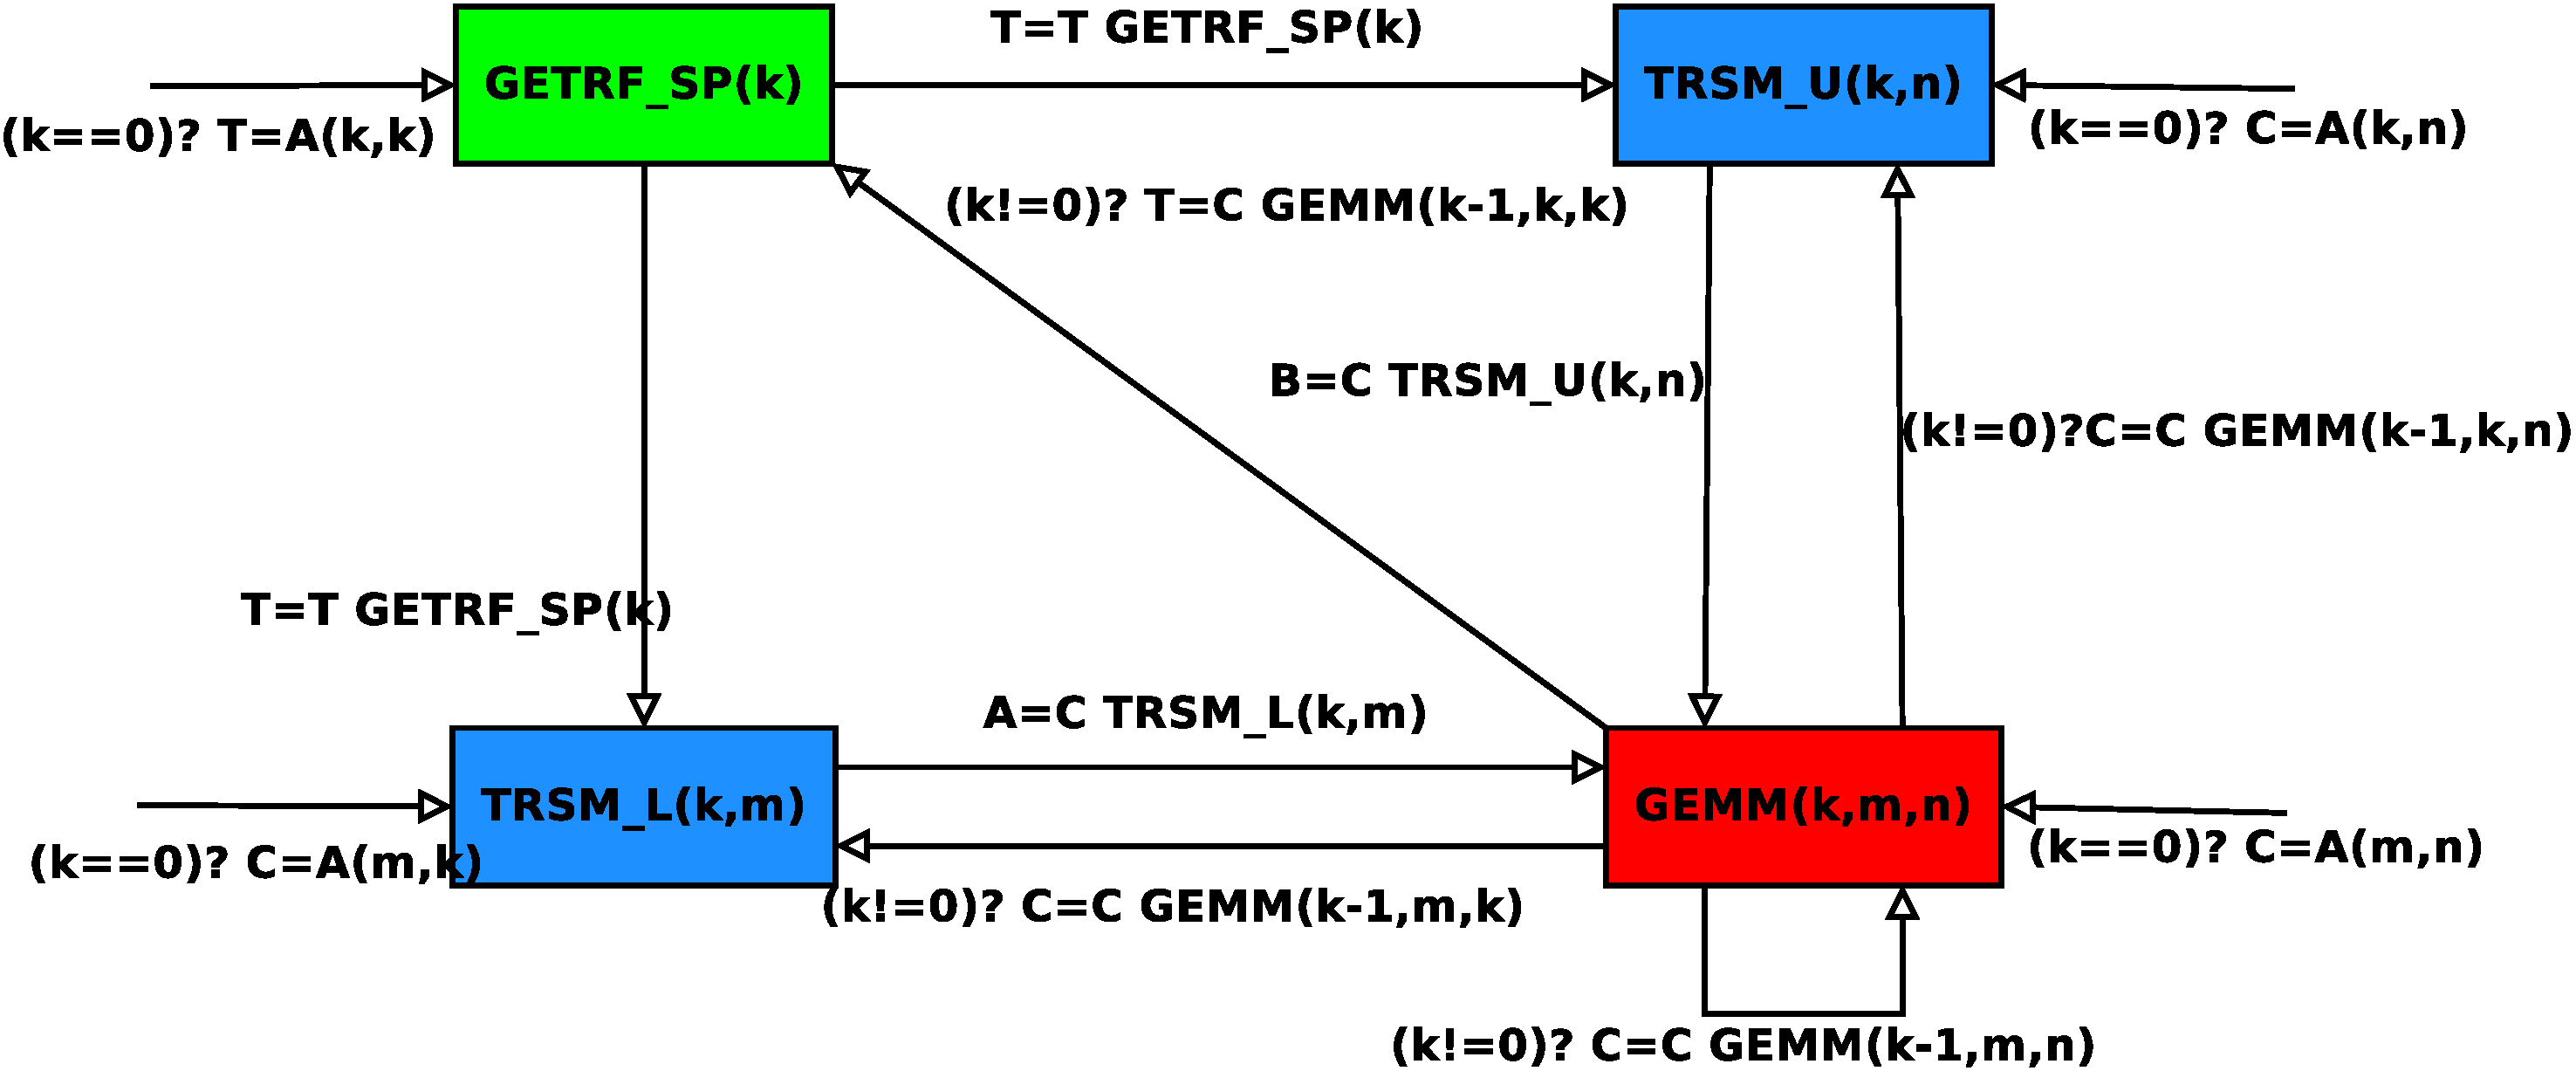
\includegraphics[scale=0.2]{dag_getrf_sp.pdf} 
\end{center}
\end{frame}

\begin{frame}{Static Pivoting}
\framesubtitle{DAG for a matrix 3*3}
\begin{center}
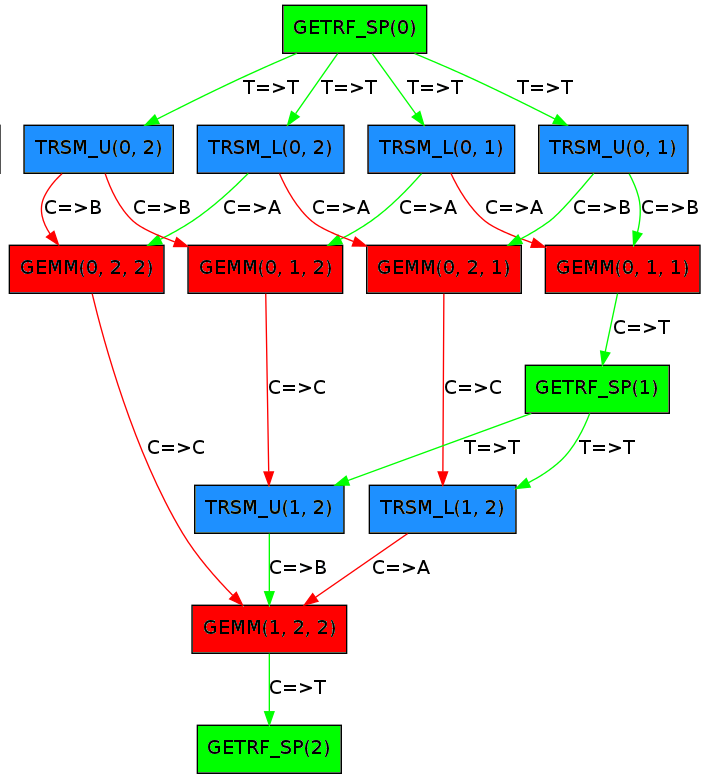
\includegraphics[width=0.5\textwidth]{dag33.png} 
\end{center}
\end{frame}



\section[Generic Update]{A generic update engine for dynamic pivoting}

\begin{frame}{A generic update engine for dynamic pivoting}
\framesubtitle{Update Issue}
\begin{columns}
\begin{column}{.50\textwidth}
\begin{center}
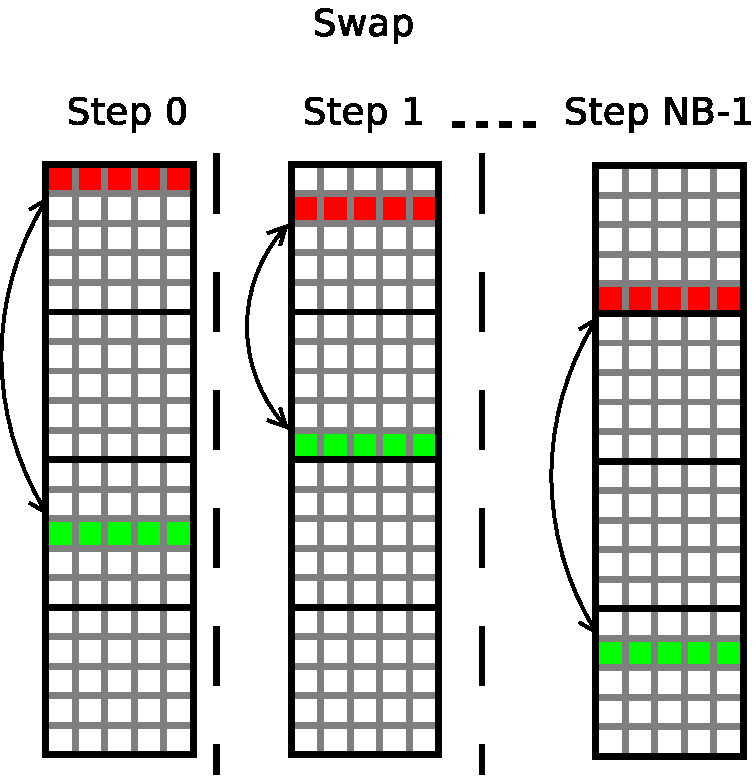
\includegraphics[scale=0.3]{update_swap.pdf}
\end{center}
\end{column}
\hfill
\begin{column}{.50\textwidth}
The tile U exchange swap rows with other concerned tile.
\pause
\begin{exampleblock}{Problem}
\begin{itemize}
\item A dynamic decision for a static DAG \\
$\rightarrow$ Prepare tasks for all possible communications?
\end{itemize}
\end{exampleblock}{}
\end{column}
\end{columns}
\end{frame}

\begin{frame}{A generic update engine for dynamic pivoting}
\framesubtitle{Solutions}
\begin{columns}
\begin{column}{.60\textwidth}
Ideas:
\begin{itemize}
\item Avoiding useless swap to increase parallelism\\
$\rightarrow$ Use of permutations instead of pivots indexes
\transparent{0.4}
\item Updating the main tile is more urgent\\
$\rightarrow$ Parallelize the swap \textbf{from} and the swap \textbf{into} the tile U
\item Minimizing the number of communication (not the volume)\\
$\rightarrow$ Gather communications of all rows over two buffers
\end{itemize}
\end{column}
\begin{column}{.40\textwidth}
\begin{center}
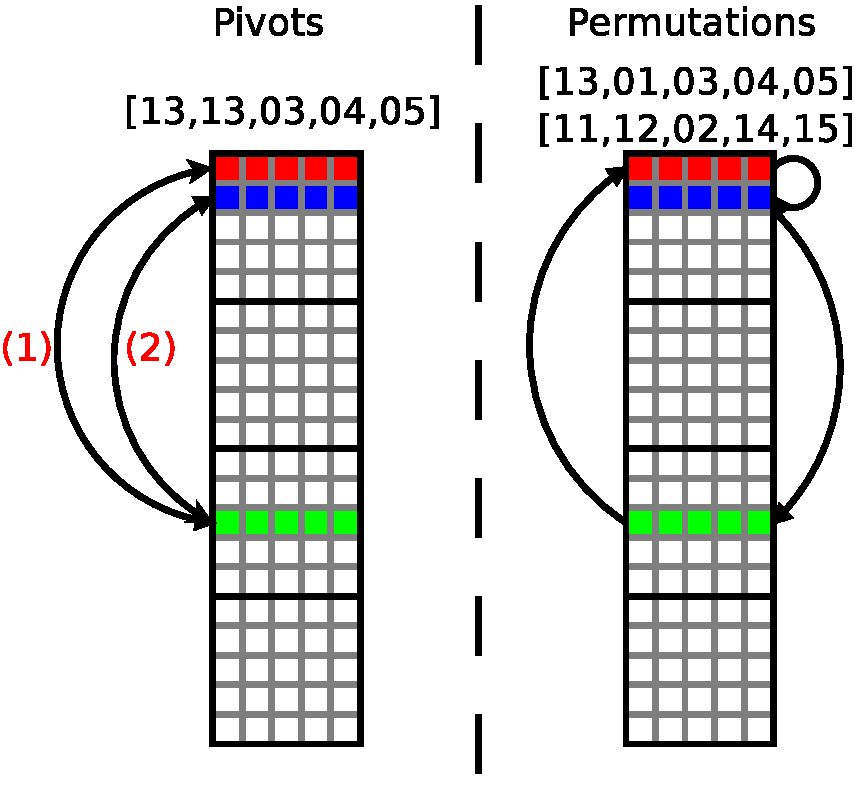
\includegraphics[scale=0.3]{pivots.pdf}
\end{center}
\end{column}
\end{columns}
\end{frame}

\begin{frame}{A generic update engine for dynamic pivoting}
\framesubtitle{Solutions}
\begin{columns}
\begin{column}{.60\textwidth}
Ideas:
\begin{itemize}
{\transparent{0.4}
\item Avoiding useless swap to increase parallelism\\
$\rightarrow$ Use of permutations instead of pivots indexes}
\item Updating the main tile is more urgent\\
$\rightarrow$ Parallelize the swap \textbf{from} and the swap \textbf{into} the tile U
\transparent{0.4}
\item Minimizing the number of communication (not the volume)\\
$\rightarrow$ Gather communications of all rows over two buffers
\end{itemize}
\end{column}
\begin{column}{.40\textwidth}
\begin{center}
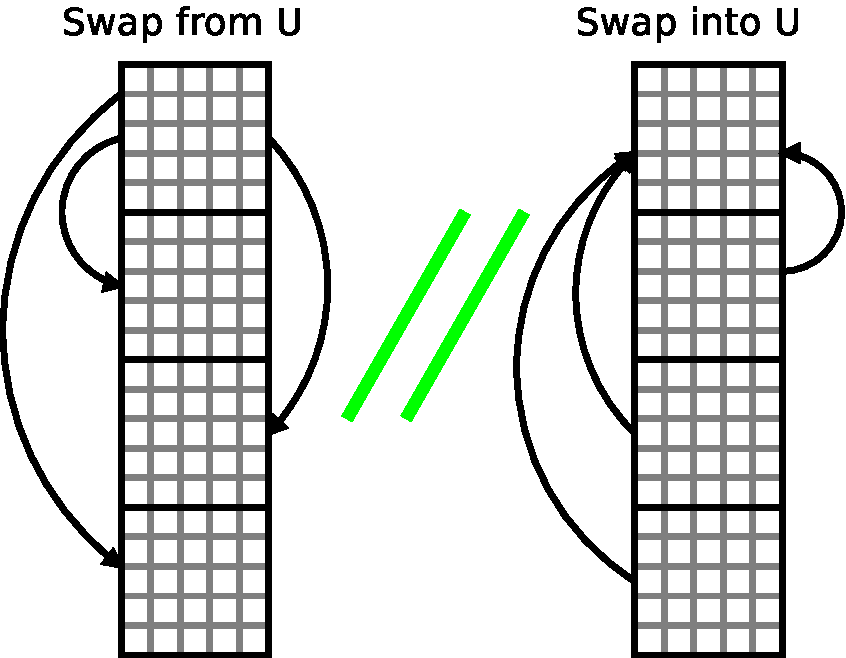
\includegraphics[scale=0.3]{parswap.pdf}
\end{center}
\end{column}
\end{columns}
\end{frame}

\begin{frame}{A generic update engine for dynamic pivoting}
\framesubtitle{Solutions}
Ideas:
\begin{itemize}
\item Avoiding useless swap to increase parallelism\\
$\rightarrow$ Use of permutations instead of pivots indexes
\item Updating the main tile is more urgent\\
$\rightarrow$ Parallelize the swap \textbf{from} and the swap \textbf{into} the tile U
\item Minimizing the number of communication (not the volume)\\
$\rightarrow$ Gather communications of all rows over two buffers
\end{itemize}
\pause
\begin{exampleblock}{}
$\rightarrow$ Five kinds of tasks : COPY, COLLECT, RECEIVE, SEND and PASTE.
\end{exampleblock}{}
\end{frame}

\begin{frame}{A generic update engine for dynamic pivoting}
\framesubtitle{Swap into U}
\begin{columns}
\begin{column}{.60\textwidth}
\begin{itemize}
\item COLLECT: Collecting the lines needed by the tile U into a buffer.
\item SEND: Gather the buffers collected by COLLECT of each node.
\item PASTE: Overwrite the tile U with the buffer.
\transparent{0.4}
\item RECEIVE
\item COPY
\end{itemize}
\end{column}
\hfill
\begin{column}{.40\textwidth}
\begin{center}
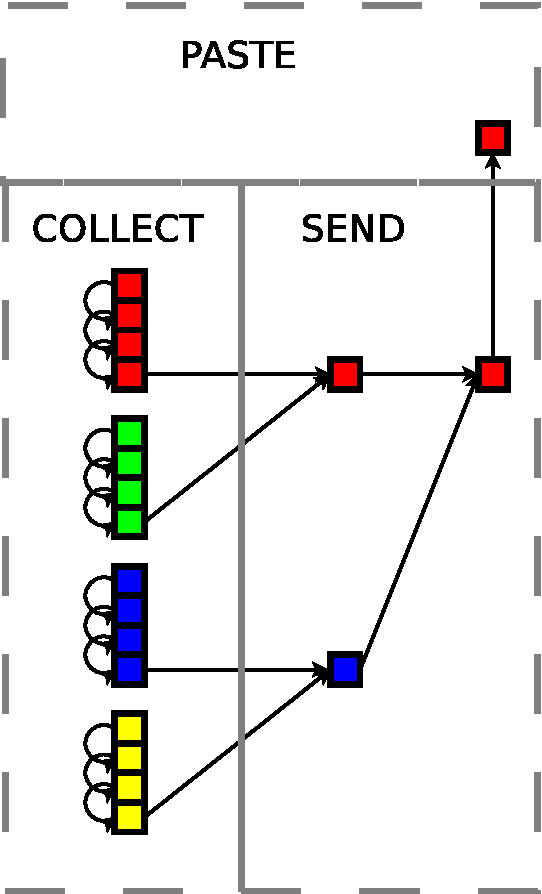
\includegraphics[scale=0.3]{collect.pdf}
\end{center}
\end{column}
\end{columns}
\end{frame}

\begin{frame}{A generic update engine for dynamic pivoting}
\framesubtitle{Swap from U}
\begin{columns}
\begin{column}{.60\textwidth}
\begin{itemize}
{
\transparent{0.4}
\item COLLECT
\item SEND
\item PASTE
}
\item COPY: Copy tile U into a buffer.
\item RECEIVE: Receive the buffer U and make the swap from it.
\end{itemize}
\end{column}
\hfill
\begin{column}{.40\textwidth}
\begin{center}
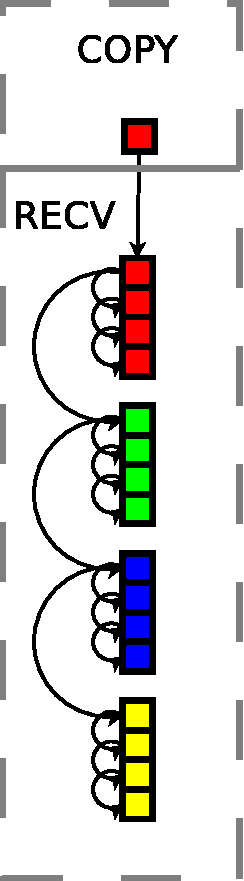
\includegraphics[scale=0.3]{receive.pdf}
\end{center}
\end{column}
\end{columns}
\end{frame}

\begin{frame}{A generic update engine for dynamic pivoting}
\framesubtitle{Update Tasks Synchronisation}
\begin{columns}
\begin{column}{.60\textwidth}
\begin{itemize}
\item COLLECT
\item COPY
\item RECEIVE
\item SEND
\item PASTE
\end{itemize}
\end{column}
\hfill
\begin{column}{.40\textwidth}
\begin{center}
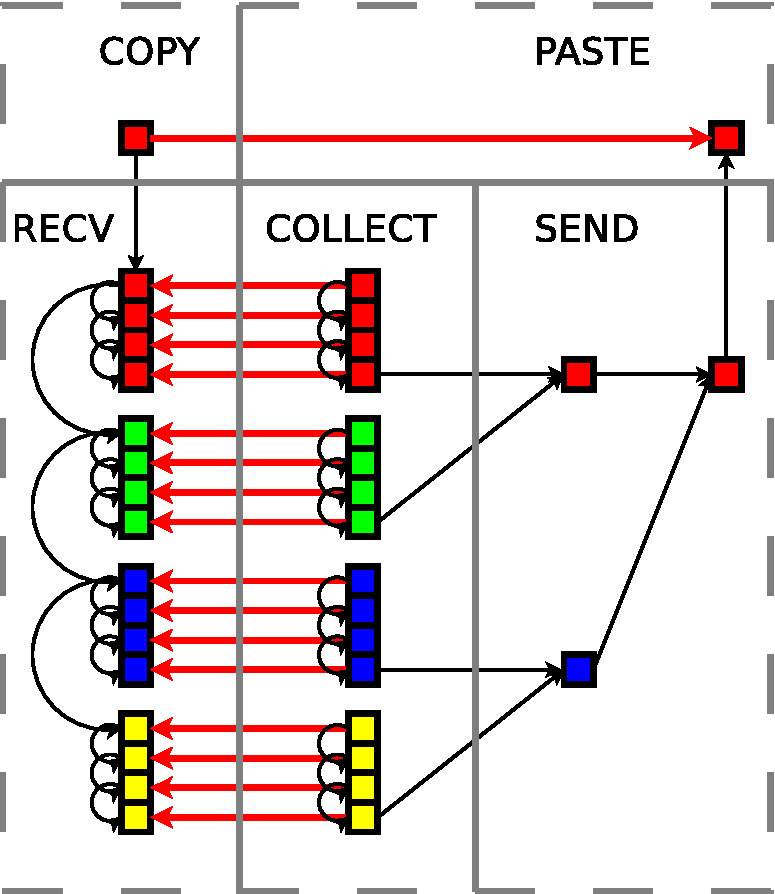
\includegraphics[scale=0.3]{swap_opt.pdf}
\end{center}
\end{column}
\end{columns}
The red arrows prevent the \alert{\textbf{READ AFTER WRITE}}.
\end{frame}

\begin{frame}{A generic update engine for dynamic pivoting}
\framesubtitle{Update Impact}
\begin{center}
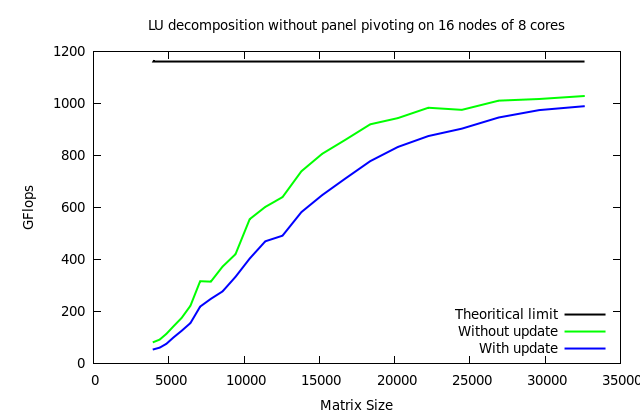
\includegraphics[width=0.7\textwidth]{dgetrf_update_problem.png} 
\end{center}
\end{frame}

\begin{frame}{A generic update engine for dynamic pivoting}
\framesubtitle{Results}
\begin{itemize}
\item Small impact on the performance
\item A generic update engine
\end{itemize}
\end{frame}

\section{Partial Pivoting}
\begin{frame}{Partial Pivoting}
\framesubtitle{Heuristic Factorization}
Several heuristic to factorize the panel:
\begin{itemize}
\item Partial pivoting
\item Threshold pivoting
\item Tournament pivoting
\begin{itemize}
\item Internal partial pivoting
\item Panel rank revealing
\end{itemize}
\end{itemize}
\end{frame}


\begin{frame}{Partial Pivoting}
\framesubtitle{Operations of Panel LU Decomposition}
\begin{center}
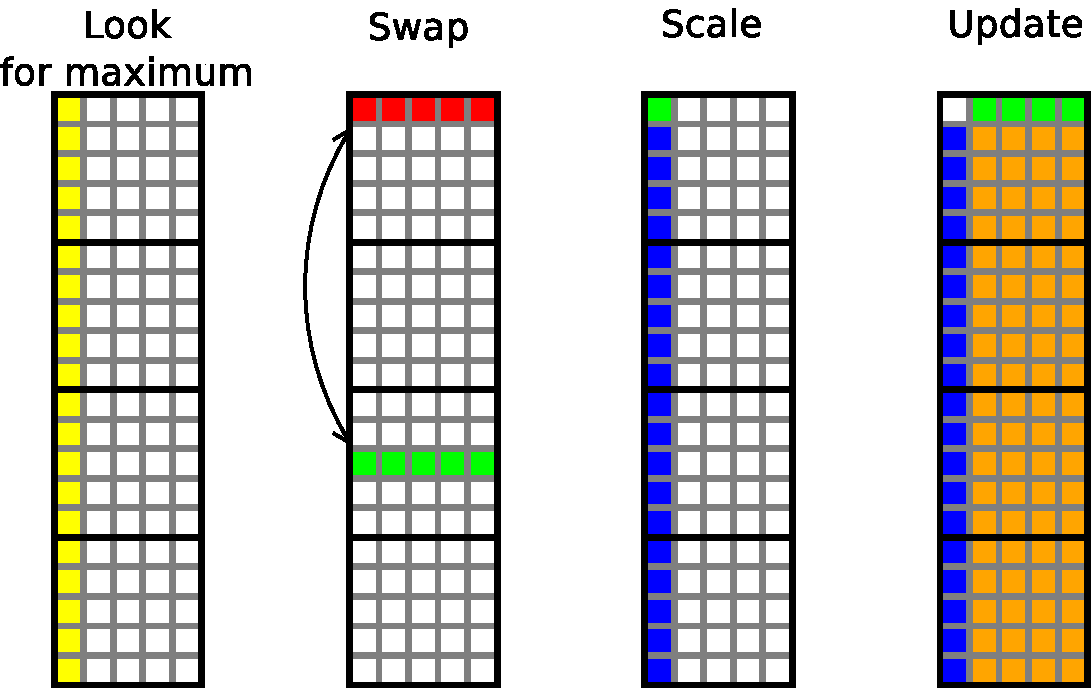
\includegraphics[scale=0.3]{panel_operation.pdf}
\end{center}
\pause
\begin{exampleblock}{Problem for implementing with task flow model is based on}
\begin{itemize}
\item Swap line is dynamically decided but the DAG is static
\item Minimize latency for the panel
\end{itemize}
\end{exampleblock}{}
\end{frame}



\begin{frame}{Partial Pivoting}
\framesubtitle{Solutions}
\begin{columns}
\begin{column}{.60\textwidth}
Solutions:
\begin{itemize}
\item Start looking for the maximum locally then reduce locally the result
\transparent{0.4}
\item Share the global result by using Bruck's algorithm
\item Use internal blocking
\end{itemize}
\end{column}
\hfill
\begin{column}{.30\textwidth}
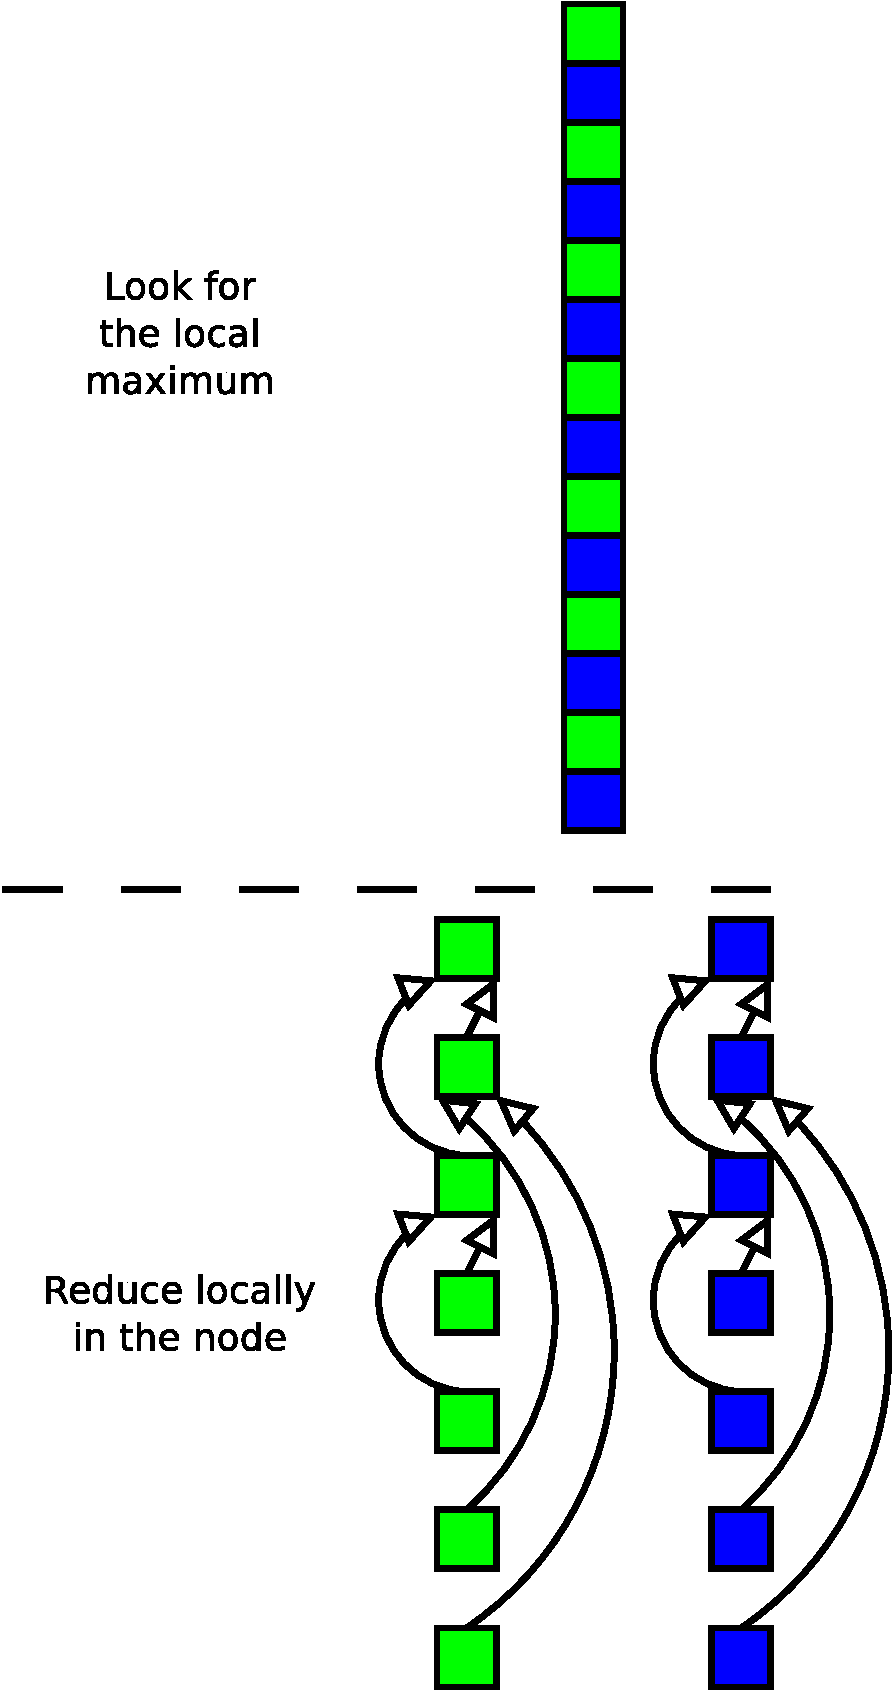
\includegraphics[scale=0.2]{binary_reduction.pdf}
\end{column}
\end{columns}
\end{frame}

\begin{frame}{Partial Pivoting}
\framesubtitle{Implemented version}
\begin{columns}
\begin{column}{.60\textwidth}
Solutions:
\begin{itemize}
{\transparent{0.4}
\item Start looking for the maximum locally then reduce locally the result
}
\item Share the global result by using Bruck's algorithm
\transparent{0.4}
\item Use internal blocking
\end{itemize}
\end{column}
\hfill
\begin{column}{.30\textwidth}
\begin{center}
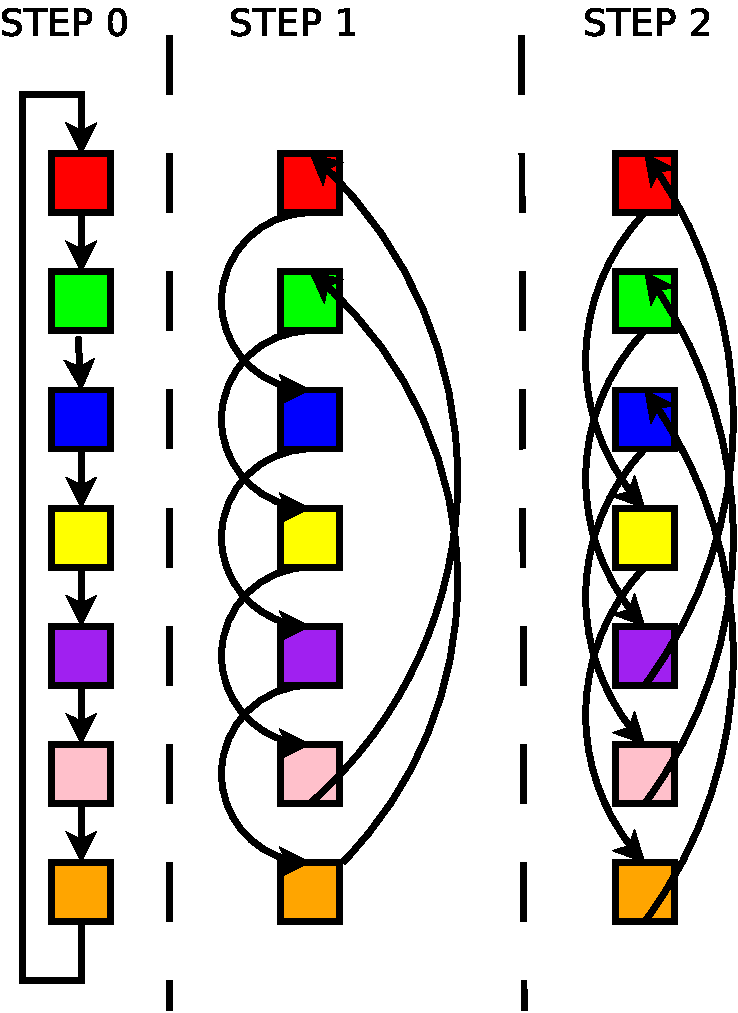
\includegraphics[scale=0.3]{bruck.pdf}
\end{center}
\end{column}
\end{columns}
\end{frame}

\begin{frame}{Partial Pivoting}
\framesubtitle{Implemented version}
\begin{columns}
\begin{column}{.50\textwidth}
Optimizations:
\begin{itemize}
{\transparent{0.4}
\item Start looking for the maximum locally then reduce locally the result
\item Share the global result by using Bruck's algorithm}
\item Use internal blocking
\end{itemize}
\end{column}
\hfill
\begin{column}{.50\textwidth}
\begin{center}
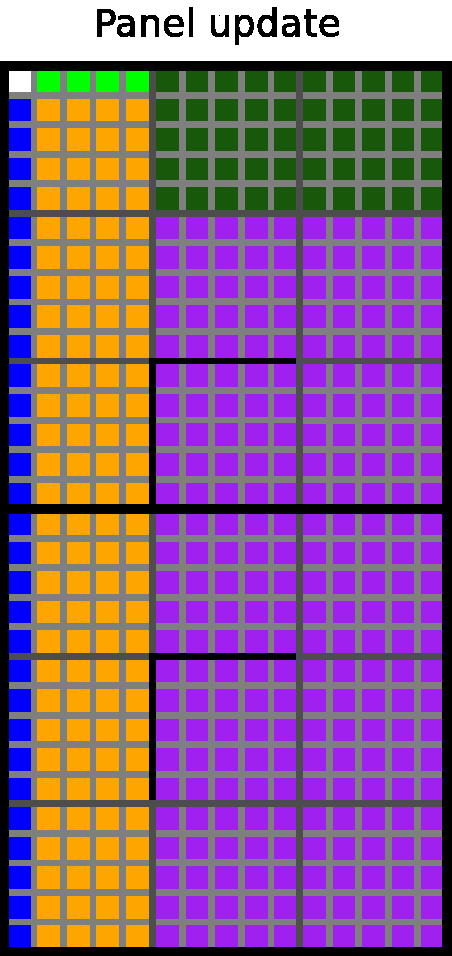
\includegraphics[scale=0.3]{panel_update.pdf}
\end{center}
\end{column}
\end{columns}
\end{frame}




\section{Performances}
\begin{frame}{Performances of partial pivoting}
\begin{itemize}
\item Shared memory
\item Problem scalability
\item Strong scalability
\end{itemize}
\end{frame}

\section*{Conclusion}
\begin{frame}{Conclusion and future work}
\end{frame}

\end{document}
